\documentclass{report}

%%%%%%%%%%%%%%%%%%%%%%%%%%%%%%%%
% PACKAGE IMPORTS
%%%%%%%%%%%%%%%%%%%%%%%%%%%%%%%%%


\usepackage[tmargin=2cm,rmargin=1in,lmargin=1in,margin=0.85in,bmargin=2cm,footskip=.2in]{geometry}
\usepackage{amsmath,amsfonts,amsthm,amssymb,mathtools}
\usepackage[varbb]{newpxmath}
\usepackage{xfrac}
\usepackage[makeroom]{cancel}
\usepackage{mathtools}
\usepackage{bookmark}
\usepackage{enumitem}
\usepackage{hyperref,theoremref}
\hypersetup{
	pdftitle={Assignment},
	colorlinks=true, linkcolor=doc!90,
	bookmarksnumbered=true,
	bookmarksopen=true
}
\usepackage[most,many,breakable]{tcolorbox}
\usepackage{xcolor}
\usepackage{varwidth}
\usepackage{varwidth}
\usepackage{etoolbox}
%\usepackage{authblk}
\usepackage{nameref}
\usepackage{multicol,array}
\usepackage{tikz-cd}
\usepackage{tikz-3dplot}
\usepackage[ruled,vlined,linesnumbered]{algorithm2e}
\usepackage{comment} % enables the use of multi-line comments (\ifx \fi) 
\usepackage{import}
\usepackage{xifthen}
\usepackage{pdfpages}
\usepackage{transparent}
\usepackage{graphicx} % <-- Added package to handle graphics
\usepackage{xcolor}
\usepackage{pgfplots}
\usepackage{minted}
\definecolor{pastelFDF7C3}{HTML}{FDF7C3}
\pgfplotsset{compat=newest}
\usepgfplotslibrary{colormaps}


\newcommand\mycommfont[1]{\footnotesize\ttfamily\textcolor{blue}{#1}}
\SetCommentSty{mycommfont}
\newcommand{\incfig}[1]{%
    \def\svgwidth{\columnwidth}
    \import{./figures/}{#1.pdf_tex}
}

\usepackage{tikzsymbols}
\renewcommand\qedsymbol{$\Laughey$}


%\usepackage{import}
%\usepackage{xifthen}
%\usepackage{pdfpages}
%\usepackage{transparent}


%%%%%%%%%%%%%%%%%%%%%%%%%%%%%%
% SELF MADE COLORS
%%%%%%%%%%%%%%%%%%%%%%%%%%%%%%



\definecolor{myg}{RGB}{56, 140, 70}
\definecolor{myb}{RGB}{45, 111, 177}
\definecolor{myr}{RGB}{199, 68, 64}
\definecolor{mytheorembg}{HTML}{F2F2F9}
\definecolor{mytheoremfr}{HTML}{00007B}
\definecolor{mylenmabg}{HTML}{FFFAF8}
\definecolor{mylenmafr}{HTML}{983b0f}
\definecolor{mypropbg}{HTML}{f2fbfc}
\definecolor{mypropfr}{HTML}{191971}
\definecolor{myexamplebg}{HTML}{F2FBF8}
\definecolor{myexamplefr}{HTML}{88D6D1}
\definecolor{myexampleti}{HTML}{2A7F7F}
\definecolor{mydefinitbg}{HTML}{E5E5FF}
\definecolor{mydefinitfr}{HTML}{3F3FA3}
\definecolor{notesgreen}{RGB}{0,162,0}
\definecolor{myp}{RGB}{197, 92, 212}
\definecolor{mygr}{HTML}{2C3338}
\definecolor{myred}{RGB}{127,0,0}
\definecolor{myyellow}{RGB}{169,121,69}
\definecolor{myexercisebg}{HTML}{F2FBF8}
\definecolor{myexercisefg}{HTML}{88D6D1}


%%%%%%%%%%%%%%%%%%%%%%%%%%%%
% TCOLORBOX SETUPS
%%%%%%%%%%%%%%%%%%%%%%%%%%%%

\setlength{\parindent}{1cm}
%================================
% THEOREM BOX
%================================

\tcbuselibrary{theorems,skins,hooks}
\newtcbtheorem[number within=section]{Theorem}{Theorem}
{%
	enhanced,
	breakable,
	colback = mytheorembg,
	frame hidden,
	boxrule = 0sp,
	borderline west = {2pt}{0pt}{mytheoremfr},
	sharp corners,
	detach title,
	before upper = \tcbtitle\par\smallskip,
	coltitle = mytheoremfr,
	fonttitle = \bfseries\sffamily,
	description font = \mdseries,
	separator sign none,
	segmentation style={solid, mytheoremfr},
}
{th}

\tcbuselibrary{theorems,skins,hooks}
\newtcbtheorem[number within=chapter]{theorem}{Theorem}
{%
	enhanced,
	breakable,
	colback = mytheorembg,
	frame hidden,
	boxrule = 0sp,
	borderline west = {2pt}{0pt}{mytheoremfr},
	sharp corners,
	detach title,
	before upper = \tcbtitle\par\smallskip,
	coltitle = mytheoremfr,
	fonttitle = \bfseries\sffamily,
	description font = \mdseries,
	separator sign none,
	segmentation style={solid, mytheoremfr},
}
{th}


\tcbuselibrary{theorems,skins,hooks}
\newtcolorbox{Theoremcon}
{%
	enhanced
	,breakable
	,colback = mytheorembg
	,frame hidden
	,boxrule = 0sp
	,borderline west = {2pt}{0pt}{mytheoremfr}
	,sharp corners
	,description font = \mdseries
	,separator sign none
}

%================================
% Corollery
%================================
\tcbuselibrary{theorems,skins,hooks}
\newtcbtheorem[number within=section]{Corollary}{Corollary}
{%
	enhanced
	,breakable
	,colback = myp!10
	,frame hidden
	,boxrule = 0sp
	,borderline west = {2pt}{0pt}{myp!85!black}
	,sharp corners
	,detach title
	,before upper = \tcbtitle\par\smallskip
	,coltitle = myp!85!black
	,fonttitle = \bfseries\sffamily
	,description font = \mdseries
	,separator sign none
	,segmentation style={solid, myp!85!black}
}
{th}
\tcbuselibrary{theorems,skins,hooks}
\newtcbtheorem[number within=chapter]{corollary}{Corollary}
{%
	enhanced
	,breakable
	,colback = myp!10
	,frame hidden
	,boxrule = 0sp
	,borderline west = {2pt}{0pt}{myp!85!black}
	,sharp corners
	,detach title
	,before upper = \tcbtitle\par\smallskip
	,coltitle = myp!85!black
	,fonttitle = \bfseries\sffamily
	,description font = \mdseries
	,separator sign none
	,segmentation style={solid, myp!85!black}
}
{th}


%================================
% LENMA
%================================

\tcbuselibrary{theorems,skins,hooks}
\newtcbtheorem[number within=section]{Lenma}{Lenma}
{%
	enhanced,
	breakable,
	colback = mylenmabg,
	frame hidden,
	boxrule = 0sp,
	borderline west = {2pt}{0pt}{mylenmafr},
	sharp corners,
	detach title,
	before upper = \tcbtitle\par\smallskip,
	coltitle = mylenmafr,
	fonttitle = \bfseries\sffamily,
	description font = \mdseries,
	separator sign none,
	segmentation style={solid, mylenmafr},
}
{th}

\tcbuselibrary{theorems,skins,hooks}
\newtcbtheorem[number within=chapter]{lenma}{Lenma}
{%
	enhanced,
	breakable,
	colback = mylenmabg,
	frame hidden,
	boxrule = 0sp,
	borderline west = {2pt}{0pt}{mylenmafr},
	sharp corners,
	detach title,
	before upper = \tcbtitle\par\smallskip,
	coltitle = mylenmafr,
	fonttitle = \bfseries\sffamily,
	description font = \mdseries,
	separator sign none,
	segmentation style={solid, mylenmafr},
}
{th}


%================================
% PROPOSITION
%================================

\tcbuselibrary{theorems,skins,hooks}
\newtcbtheorem[number within=section]{Prop}{Proposition}
{%
	enhanced,
	breakable,
	colback = mypropbg,
	frame hidden,
	boxrule = 0sp,
	borderline west = {2pt}{0pt}{mypropfr},
	sharp corners,
	detach title,
	before upper = \tcbtitle\par\smallskip,
	coltitle = mypropfr,
	fonttitle = \bfseries\sffamily,
	description font = \mdseries,
	separator sign none,
	segmentation style={solid, mypropfr},
}
{th}

\tcbuselibrary{theorems,skins,hooks}
\newtcbtheorem[number within=chapter]{prop}{Proposition}
{%
	enhanced,
	breakable,
	colback = mypropbg,
	frame hidden,
	boxrule = 0sp,
	borderline west = {2pt}{0pt}{mypropfr},
	sharp corners,
	detach title,
	before upper = \tcbtitle\par\smallskip,
	coltitle = mypropfr,
	fonttitle = \bfseries\sffamily,
	description font = \mdseries,
	separator sign none,
	segmentation style={solid, mypropfr},
}
{th}


%================================
% CLAIM
%================================

\tcbuselibrary{theorems,skins,hooks}
\newtcbtheorem[number within=section]{claim}{Claim}
{%
	enhanced
	,breakable
	,colback = myg!10
	,frame hidden
	,boxrule = 0sp
	,borderline west = {2pt}{0pt}{myg}
	,sharp corners
	,detach title
	,before upper = \tcbtitle\par\smallskip
	,coltitle = myg!85!black
	,fonttitle = \bfseries\sffamily
	,description font = \mdseries
	,separator sign none
	,segmentation style={solid, myg!85!black}
}
{th}



%================================
% Exercise
%================================

\tcbuselibrary{theorems,skins,hooks}
\newtcbtheorem[number within=section]{Exercise}{Exercise}
{%
	enhanced,
	breakable,
	colback = myexercisebg,
	frame hidden,
	boxrule = 0sp,
	borderline west = {2pt}{0pt}{myexercisefg},
	sharp corners,
	detach title,
	before upper = \tcbtitle\par\smallskip,
	coltitle = myexercisefg,
	fonttitle = \bfseries\sffamily,
	description font = \mdseries,
	separator sign none,
	segmentation style={solid, myexercisefg},
}
{th}

\tcbuselibrary{theorems,skins,hooks}
\newtcbtheorem[number within=chapter]{exercise}{Exercise}
{%
	enhanced,
	breakable,
	colback = myexercisebg,
	frame hidden,
	boxrule = 0sp,
	borderline west = {2pt}{0pt}{myexercisefg},
	sharp corners,
	detach title,
	before upper = \tcbtitle\par\smallskip,
	coltitle = myexercisefg,
	fonttitle = \bfseries\sffamily,
	description font = \mdseries,
	separator sign none,
	segmentation style={solid, myexercisefg},
}
{th}

%================================
% EXAMPLE BOX (Lighter Pastel Purple)
%================================

\definecolor{pastelExampleBg}{HTML}{70AF85} % Base pastel color
\definecolor{greenPast}{HTML}{86C8BC} % Base pastel color
\colorlet{myexamplebg}{pastelExampleBg!25!white} % Mix with white for a pastel color
\colorlet{myexamplefr}{pastelExampleBg!85!white} % Use the same mix for the frame
\colorlet{myexampleti}{greenPast!40!black} % Mix A1EEBD with black for a darker green

\newtcbtheorem[number within=section]{Example}{Example}
{%
	colback = myexamplebg
	,breakable
	,colframe = myexamplefr
	,coltitle = myexampleti
	,boxrule = 1pt
	,sharp corners
	,detach title
	,before upper=\tcbtitle\par\smallskip
	,fonttitle = \bfseries
	,description font = \mdseries
	,separator sign none
	,description delimiters parenthesis
}
{ex}

\newtcbtheorem[number within=chapter]{example}{Example}
{%
	colback = myexamplebg
	,breakable
	,colframe = myexamplefr
	,coltitle = myexampleti
	,boxrule = 1pt
	,sharp corners
	,detach title
	,before upper=\tcbtitle\par\smallskip
	,fonttitle = \bfseries
	,description font = \mdseries
	,separator sign none
	,description delimiters parenthesis
}
{ex}

%================================
% EXAMPLE BOX (Rose)
%================================

% Define the custom example box with rose image in the top-right corner
\newtcolorbox[auto counter, number within=section]{ExampleWithRose}[2][]{%
    colback=myexamplebg,  % Use the pastel version of BFF6C3 for the background
    colframe=myexamplefr, % Use the pastel version of BFF6C3 for the frame
    coltitle=myexampleti, % Use black for the title color
    fonttitle=\bfseries,
    title={Example~\thetcbcounter: #2},
    sharp corners,
    enhanced,
    overlay={
        \node[anchor=south east] at (frame.south east) {
\includegraphics[width=1.5cm]{flow.png}};
    },
    #1
}

%================================
% DEFINITION BOX
%================================

\makeatletter
\definecolor{customblue}{RGB}{198, 220, 228} % Custom blue color
\definecolor{darkblue}{RGB}{90, 120, 140} % Darker blue for text

\newtcbtheorem[number within=section]{Definition}{Definition}{enhanced,
	before skip=2mm,after skip=2mm, colback=customblue!20,colframe=customblue!80,boxrule=0.5mm,
	attach boxed title to top left={xshift=1cm,yshift*=1mm-\tcboxedtitleheight}, varwidth boxed title*=-3cm,
	boxed title style={frame code={
					\path[fill=customblue]  % Custom blue fill
					([yshift=-1mm,xshift=-1mm]frame.north west)
					arc[start angle=0,end angle=180,radius=1mm]
					([yshift=-1mm,xshift=1mm]frame.north east)
					arc[start angle=180,end angle=0,radius=1mm];
					\path[left color=customblue,right color=customblue,
						middle color=customblue!90]  % Light custom blue gradient
					([xshift=-2mm]frame.north west) -- ([xshift=2mm]frame.north east)
					[rounded corners=1mm]-- ([xshift=1mm,yshift=-1mm]frame.north east)
					-- (frame.south east) -- (frame.south west)
					-- ([xshift=-1mm,yshift=-1mm]frame.north west)
					[sharp corners]-- cycle;
				},interior engine=empty,
		},
	fonttitle=\bfseries\color{darkblue}, % Darker blue for the title text
	coltitle=darkblue, % Darker blue for the box title
	colbacktitle=customblue!80, % Background for the title
	title={#2},#1}{def}

\newtcbtheorem[number within=chapter]{definition}{Definition}{enhanced,
	before skip=2mm,after skip=2mm, colback=customblue!20,colframe=customblue!80,boxrule=0.5mm,
	attach boxed title to top left={xshift=1cm,yshift*=1mm-\tcboxedtitleheight}, varwidth boxed title*=-3cm,
	boxed title style={frame code={
					\path[fill=customblue]  % Custom blue fill
					([yshift=-1mm,xshift=-1mm]frame.north west)
					arc[start angle=0,end angle=180,radius=1mm]
					([yshift=-1mm,xshift=1mm]frame.north east)
					arc[start angle=180,end angle=0,radius=1mm];
					\path[left color=customblue,right color=customblue,
						middle color=customblue!90]  % Light custom blue gradient
					([xshift=-2mm]frame.north west) -- ([xshift=2mm]frame.north east)
					[rounded corners=1mm]-- ([xshift=1mm,yshift=-1mm]frame.north east)
					-- (frame.south east) -- (frame.south west)
					-- ([xshift=-1mm,yshift=-1mm]frame.north west)
					[sharp corners]-- cycle;
				},interior engine=empty,
		},
	fonttitle=\bfseries\color{darkblue}, % Darker blue for the title text
	coltitle=darkblue, % Darker blue for the box title
	colbacktitle=customblue!80, % Background for the title
	title={#2},#1}{def}
\makeatother

%================================
% DEFINITION BOX WITH IMAGE IN BOTTOM-RIGHT
%================================

%================================
% DEFINITION BOX WITH IMAGE IN BOTTOM-RIGHT
%================================

\makeatletter
\definecolor{customblue}{RGB}{198, 234, 245} % Custom blue color
\definecolor{darkblue}{RGB}{90, 120, 140} % Darker blue for text

\newtcbtheorem[number within=section]{DefinitionWithImage}{Definition}{enhanced,
	before skip=2mm,
	after skip=2mm, 
	colback=customblue!40, % Use custom blue with 20% intensity for background
	colframe=customblue!80!black, % Use custom blue with some black for the frame
	boxrule=0.5mm,
	attach boxed title to top left={xshift=1cm,yshift*=1mm-\tcboxedtitleheight}, 
	varwidth boxed title*=-3cm,
	boxed title style={frame code={
					\path[fill=customblue]  % Custom blue fill
					([yshift=-1mm,xshift=-1mm]frame.north west)
					arc[start angle=0,end angle=180,radius=1mm]
					([yshift=-1mm,xshift=1mm]frame.north east)
					arc[start angle=180,end angle=0,radius=1mm];
					\path[left color=customblue,right color=customblue,
						middle color=customblue!90]  % Light custom blue gradient
					([xshift=-2mm]frame.north west) -- ([xshift=2mm]frame.north east)
					[rounded corners=1mm]-- ([xshift=1mm,yshift=-1mm]frame.north east)
					-- (frame.south east) -- (frame.south west)
					-- ([xshift=-1mm,yshift=-1mm]frame.north west)
					[sharp corners]-- cycle;
				},interior engine=empty,
		},
	fonttitle=\bfseries\color{darkblue}, % Darker blue for the title text
	coltitle=darkblue, % Darker blue for the box title
	colbacktitle=customblue!80, % Background for the title
	title={#2},
	overlay unbroken and last={
		\node[anchor=south east,xshift=-2mm,yshift=2mm] at (frame.south east) {
\includegraphics[width=1 cm]{slime.png}};
	} % Adjust the path and size to your needs
}{def}
\makeatother

%================================
% Solution BOX (Pastel Light Blue)
%================================

\makeatletter
\definecolor{pastelpink}{HTML}{FFE3ED} % Define pastel pink using the hex code #FFE3ED

\newtcbtheorem{question}{Question}{enhanced,
	breakable,
	colback=pastelpink!60, % Use pastel pink for the background with 60% intensity
	colframe=pastelpink!90!black, % Use pastel pink with a bit of black for the frame
	attach boxed title to top left={yshift*=-\tcboxedtitleheight},
	fonttitle=\bfseries,
	title={#2},
	boxed title size=title,
	boxed title style={%
			sharp corners,
			rounded corners=northwest,
			colback=tcbcolframe,
			boxrule=0pt,
		},
	underlay boxed title={%
			\path[fill=tcbcolframe] (title.south west)--(title.south east)
			to[out=0, in=180] ([xshift=5mm]title.east)--
			(title.center-|frame.east)
			[rounded corners=\kvtcb@arc] |-
			(frame.north) -| cycle;
		},
	#1
}{def}
\makeatother


% SOLUTION BOX
%================================

\makeatletter
\newtcolorbox{solution}{enhanced,
	breakable,
	colback=white,
	colframe=myg!80!black,
	attach boxed title to top left={yshift*=-\tcboxedtitleheight},
	title=Solution,
	boxed title size=title,
	boxed title style={%
			sharp corners,
			rounded corners=northwest,
			colback=tcbcolframe,
			boxrule=0pt,
		},
	underlay boxed title={%
			\path[fill=tcbcolframe] (title.south west)--(title.south east)
			to[out=0, in=180] ([xshift=5mm]title.east)--
			(title.center-|frame.east)
			[rounded corners=\kvtcb@arc] |-
			(frame.north) -| cycle;
		},
}
\makeatother

%================================
% Question BOX
%================================

\makeatletter
\newtcbtheorem{qstion}{Question}{enhanced,
	breakable,
	colback=white,
	colframe=mygr,
	attach boxed title to top left={yshift*=-\tcboxedtitleheight},
	fonttitle=\bfseries,
	title={#2},
	boxed title size=title,
	boxed title style={%
			sharp corners,
			rounded corners=northwest,
			colback=tcbcolframe,
			boxrule=0pt,
		},
	underlay boxed title={%
			\path[fill=tcbcolframe] (title.south west)--(title.south east)
			to[out=0, in=180] ([xshift=5mm]title.east)--
			(title.center-|frame.east)
			[rounded corners=\kvtcb@arc] |-
			(frame.north) -| cycle;
		},
	#1
}{def}
\makeatother

\newtcbtheorem[number within=chapter]{wconc}{Wrong Concept}{
	breakable,
	enhanced,
	colback=white,
	colframe=myr,
	arc=0pt,
	outer arc=0pt,
	fonttitle=\bfseries\sffamily\large,
	colbacktitle=myr,
	attach boxed title to top left={},
	boxed title style={
			enhanced,
			skin=enhancedfirst jigsaw,
			arc=3pt,
			bottom=0pt,
			interior style={fill=myr}
		},
	#1
}{def}



%================================
% NOTE BOX (Pastel Pink)
%================================

\usetikzlibrary{arrows,calc,shadows.blur}
\tcbuselibrary{skins}
\definecolor{pastelpink}{HTML}{FFE3ED} % Define pastel pink using the hex code #FFE3ED

\newtcolorbox{note}[1][]{%
    enhanced jigsaw,
    colback=pastelpink, % Use pastel pink for the background
    colframe=pastelpink, % Use pastel pink for the frame
    size=small,
    boxrule=1pt,
    title=\textbf{Note:-},
    halign title=flush center,
    coltitle=black,
    breakable,
    drop shadow=black!50!white,
    attach boxed title to top left={xshift=1cm,yshift=-\tcboxedtitleheight/2,yshifttext=-\tcboxedtitleheight/2},
    minipage boxed title=1.5cm,
    boxed title style={%
            colback=white,
            size=fbox,
            boxrule=1pt,
            boxsep=2pt,
            underlay={%
                    \coordinate (dotA) at ($(interior.west) + (-0.5pt,0)$);
                    \coordinate (dotB) at ($(interior.east) + (0.5pt,0)$);
                    \begin{scope}
                        \clip (interior.north west) rectangle ([xshift=3ex]interior.east);
                        \filldraw [white, blur shadow={shadow opacity=60, shadow yshift=-.75ex}, rounded corners=2pt] (interior.north west) rectangle (interior.south east);
                    \end{scope}
                    \begin{scope}[pastelpink]
                        \fill (dotA) circle (2pt);
                        \fill (dotB) circle (2pt);
                    \end{scope}
                },
        },
    #1,
}

%================================
% NOTE BOX (Pastel Pink with Image in Bottom-Left)
%================================
\newtcolorbox{noteWithImage}[1][]{%
    enhanced jigsaw,
    colback=pastelFDF7C3!70!white, % Mix pastelFDF7C3 with white to lighten the color
    colframe=pastelFDF7C3!80!white, % Mix pastelFDF7C3 with white for the frame
    size=small,
    boxrule=1pt,
    title=\textbf{Note:-},
    halign title=flush center,
    coltitle=black,
    breakable,
    drop shadow=black!50!white,
    attach boxed title to top left={xshift=1cm,yshift=-\tcboxedtitleheight/2,yshifttext=-\tcboxedtitleheight/2},
    minipage boxed title=1.5cm,
    boxed title style={%
            colback=white,
            size=fbox,
            boxrule=1pt,
            boxsep=2pt,
            underlay={%
                    \coordinate (dotA) at ($(interior.west) + (-0.5pt,0)$);
                    \coordinate (dotB) at ($(interior.east) + (0.5pt,0)$);
                    \begin{scope}
                        \clip (interior.north west) rectangle ([xshift=3ex]interior.east);
                        \filldraw [white, blur shadow={shadow opacity=60, shadow yshift=-.75ex}, rounded corners=2pt] (interior.north west) rectangle (interior.south east);
                    \end{scope}
                    \begin{scope}[pastelFDF7C3!80!white]
                        \fill (dotA) circle (2pt);
                        \fill (dotB) circle (2pt);
                    \end{scope}
                },
        },
    overlay unbroken and last={
        \node[anchor=south east,xshift=-2mm,yshift=1mm] at (frame.south east) {
\includegraphics[width=1cm]{lot.png}};
    }, % Replace 'rose.png' with the path to your image
    #1,
}


%%%%%%%%%%%%%%%%%%%%%%%%%%%%%%
% SELF MADE COMMANDS
%%%%%%%%%%%%%%%%%%%%%%%%%%%%%%


\newcommand{\thm}[2]{\begin{Theorem}{#1}{}#2\end{Theorem}}
\newcommand{\cor}[2]{\begin{Corollary}{#1}{}#2\end{Corollary}}
\newcommand{\mlenma}[2]{\begin{Lenma}{#1}{}#2\end{Lenma}}
\newcommand{\mprop}[2]{\begin{Prop}{#1}{}#2\end{Prop}}
\newcommand{\clm}[3]{\begin{claim}{#1}{#2}#3\end{claim}}
\newcommand{\wc}[2]{\begin{wconc}{#1}{}\setlength{\parindent}{1cm}#2\end{wconc}}
\newcommand{\thmcon}[1]{\begin{Theoremcon}{#1}\end{Theoremcon}}
\newcommand{\exer}[2]{\begin{Exercise}{#1}{}#2\end{Exercise}}
\newcommand{\ex}[2]{\begin{Example}{#1}{}#2\end{Example}}
\newcommand{\dfn}[2]{\begin{Definition}[colbacktitle=red!75!black]{#1}{}#2\end{Definition}}
\newcommand{\dfnc}[2]{\begin{definition}[colbacktitle=red!75!black]{#1}{}#2\end{definition}}
\newcommand{\qs}[2]{\begin{question}{#1}{}#2\end{question}}
\newcommand{\pf}[2]{\begin{myproof}[#1]#2\end{myproof}}
\newcommand{\nt}[1]{\begin{note}#1\end{note}}
\newcommand{\insertpng}[2][1]{\begin{center} \includegraphics[scale=#1]{#2} \end{center}} % <-- New command for PNG insertion

\newcommand{\defrose}[2]{%
    \begin{DefinitionWithImage}{#1}%
        #2%
    \end{DefinitionWithImage}%
}

\newcommand{\exrose}[2]{%
    \begin{ExampleWithRose}{#1}%
        #2%
    \end{ExampleWithRose}%
}

\newcommand{\ntimg}[2][]{%
    \begin{noteWithImage}[#1]%
        #2%
    \end{noteWithImage}%
}

\newcommand*\circled[1]{\tikz[baseline=(char.base)]{
		\node[shape=circle,draw,inner sep=1pt] (char) {#1};}}
\newcommand\getcurrentref[1]{%
	\ifnumequal{\value{#1}}{0}
	{??}
	{\the\value{#1}}%
}
\newcommand{\getCurrentSectionNumber}{\getcurrentref{section}}
\newenvironment{myproof}[1][\proofname]{%
	\proof[\bfseries #1: ]%
}{\endproof}

\newcommand{\mclm}[2]{\begin{myclaim}[#1]#2\end{myclaim}}
\newenvironment{myclaim}[1][\claimname]{\proof[\bfseries #1: ]}{}

\newcounter{mylabelcounter}

\makeatletter
\newcommand{\setword}[2]{%
	\phantomsection
	#1\def\@currentlabel{\unexpanded{#1}}\label{#2}%
}
\makeatother




\tikzset{
	symbol/.style={
			draw=none,
			every to/.append style={
					edge node={node [sloped, allow upside down, auto=false]{$#1$}}}
		}
}


% deliminators
\DeclarePairedDelimiter{\abs}{\lvert}{\rvert}
\DeclarePairedDelimiter{\norm}{\lVert}{\rVert}

\DeclarePairedDelimiter{\ceil}{\lceil}{\rceil}
\DeclarePairedDelimiter{\floor}{\lfloor}{\rfloor}
\DeclarePairedDelimiter{\round}{\lfloor}{\rceil}

\newsavebox\diffdbox
\newcommand{\slantedromand}{{\mathpalette\makesl{d}}}
\newcommand{\makesl}[2]{%
\begingroup
\sbox{\diffdbox}{$\mathsurround=0pt#1\mathrm{#2}$}%
\pdfsave
\pdfsetmatrix{1 0 0.2 1}%
\rlap{\usebox{\diffdbox}}%
\pdfrestore
\hskip\wd\diffdbox
\endgroup
}
\newcommand{\dd}[1][]{\ensuremath{\mathop{}\!\ifstrempty{#1}{%
\slantedromand\@ifnextchar^{\hspace{0.2ex}}{\hspace{0.1ex}}}%
{\slantedromand\hspace{0.2ex}^{#1}}}}
\ProvideDocumentCommand\dv{o m g}{%
  \ensuremath{%
    \IfValueTF{#3}{%
      \IfNoValueTF{#1}{%
        \frac{\dd #2}{\dd #3}%
      }{%
        \frac{\dd^{#1} #2}{\dd #3^{#1}}%
      }%
    }{%
      \IfNoValueTF{#1}{%
        \frac{\dd}{\dd #2}%
      }{%
        \frac{\dd^{#1}}{\dd #2^{#1}}%
      }%
    }%
  }%
}
\providecommand*{\pdv}[3][]{\frac{\partial^{#1}#2}{\partial#3^{#1}}}
%  - others
\DeclareMathOperator{\Lap}{\mathcal{L}}
\DeclareMathOperator{\Var}{Var} % varience
\DeclareMathOperator{\Cov}{Cov} % covarience
\DeclareMathOperator{\E}{E} % expected

% Since the amsthm package isn't loaded

% I prefer the slanted \leq
\let\oldleq\leq % save them in case they're every wanted
\let\oldgeq\geq
\renewcommand{\leq}{\leqslant}
\renewcommand{\geq}{\geqslant}

% % redefine matrix env to allow for alignment, use r as default
% \renewcommand*\env@matrix[1][r]{\hskip -\arraycolsep
%     \let\@ifnextchar\new@ifnextchar
%     \array{*\c@MaxMatrixCols #1}}


%\usepackage{framed}
%\usepackage{titletoc}
%\usepackage{etoolbox}
%\usepackage{lmodern}


%\patchcmd{\tableofcontents}{\contentsname}{\sffamily\contentsname}{}{}

%\renewenvironment{leftbar}
%{\def\FrameCommand{\hspace{6em}%
%		{\color{myyellow}\vrule width 2pt depth 6pt}\hspace{1em}}%
%	\MakeFramed{\parshape 1 0cm \dimexpr\textwidth-6em\relax\FrameRestore}\vskip2pt%
%}
%{\endMakeFramed}

%\titlecontents{chapter}
%[0em]{\vspace*{2\baselineskip}}
%{\parbox{4.5em}{%
%		\hfill\Huge\sffamily\bfseries\color{myred}\thecontentspage}%
%	\vspace*{-2.3\baselineskip}\leftbar\textsc{\small\chaptername~\thecontentslabel}\\\sffamily}
%{}{\endleftbar}
%\titlecontents{section}
%[8.4em]
%{\sffamily\contentslabel{3em}}{}{}
%{\hspace{0.5em}\nobreak\itshape\color{myred}\contentspage}
%\titlecontents{subsection}
%[8.4em]
%{\sffamily\contentslabel{3em}}{}{}  
%{\hspace{0.5em}\nobreak\itshape\color{myred}\contentspage}



%%%%%%%%%%%%%%%%%%%%%%%%%%%%%%%%%%%%%%%%%%%
% TABLE OF CONTENTS
%%%%%%%%%%%%%%%%%%%%%%%%%%%%%%%%%%%%%%%%%%%

\usepackage{tikz}
\definecolor{doc}{HTML}{AD6989} % Define the new color using the hex code #AD6989
\usepackage{titletoc}
\contentsmargin{0cm}
\titlecontents{chapter}[3.7pc]
{\addvspace{30pt}%
	\begin{tikzpicture}[remember picture, overlay]%
		\draw[fill=doc!60,draw=doc!60] (-7,-.1) rectangle (-0.9,.5);%
		\pgftext[left,x=-3.5cm,y=0.2cm]{\color{white}\Large\sc\bfseries Chapter\ \thecontentslabel};%
	\end{tikzpicture}\color{doc!60}\large\sc\bfseries}%
{}
{}
{\;\titlerule\;\large\sc\bfseries Page \thecontentspage
	\begin{tikzpicture}[remember picture, overlay]
		\draw[fill=doc!60,draw=doc!60] (2pt,0) rectangle (4,0.1pt);
	\end{tikzpicture}}%
\titlecontents{section}[3.7pc]
{\addvspace{2pt}}
{\contentslabel[\thecontentslabel]{2pc}}
{}
{\hfill\small \thecontentspage}
[]
\titlecontents*{subsection}[3.7pc]
{\addvspace{-1pt}\small}
{}
{}
{\ --- \small\thecontentspage}
[ \textbullet\ ][]

\makeatletter
\renewcommand{\tableofcontents}{%
	\chapter*{%
	  \vspace*{-20\p@}%
	  \begin{tikzpicture}[remember picture, overlay]%
		  \pgftext[right,x=15cm,y=0.2cm]{\color{doc!60}\Huge\sc\bfseries \contentsname};%
		  \draw[fill=doc!60,draw=doc!60] (13,-.75) rectangle (20,1);%
		  \clip (13,-.75) rectangle (20,1);
		  \pgftext[right,x=15cm,y=0.2cm]{\color{white}\Huge\sc\bfseries \contentsname};%
	  \end{tikzpicture}}%
	\@starttoc{toc}}
\makeatother

%From M275 "Topology" at SJSU
\newcommand{\id}{\mathrm{id}}
\newcommand{\taking}[1]{\xrightarrow{#1}}
\newcommand{\inv}{^{-1}}

%From M170 "Introduction to Graph Theory" at SJSU
\DeclareMathOperator{\diam}{diam}
\DeclareMathOperator{\ord}{ord}
\newcommand{\defeq}{\overset{\mathrm{def}}{=}}

%From the USAMO .tex files
\newcommand{\ts}{\textsuperscript}
\newcommand{\dg}{^\circ}
\newcommand{\ii}{\item}

% % From Math 55 and Math 145 at Harvard
% \newenvironment{subproof}[1][Proof]{%
% \begin{proof}[#1] \renewcommand{\qedsymbol}{$\blacksquare$}}%
% {\end{proof}}

\newcommand{\liff}{\leftrightarrow}
\newcommand{\lthen}{\rightarrow}
\newcommand{\opname}{\operatorname}
\newcommand{\surjto}{\twoheadrightarrow}
\newcommand{\injto}{\hookrightarrow}
\newcommand{\On}{\mathrm{On}} % ordinals
\DeclareMathOperator{\img}{im} % Image
\DeclareMathOperator{\Img}{Im} % Image
\DeclareMathOperator{\coker}{coker} % Cokernel
\DeclareMathOperator{\Coker}{Coker} % Cokernel
\DeclareMathOperator{\Ker}{Ker} % Kernel
\DeclareMathOperator{\rank}{rank}
\DeclareMathOperator{\Spec}{Spec} % spectrum
\DeclareMathOperator{\Tr}{Tr} % trace
\DeclareMathOperator{\pr}{pr} % projection
\DeclareMathOperator{\ext}{ext} % extension
\DeclareMathOperator{\pred}{pred} % predecessor
\DeclareMathOperator{\dom}{dom} % domain
\DeclareMathOperator{\ran}{ran} % range
\DeclareMathOperator{\Hom}{Hom} % homomorphism
\DeclareMathOperator{\Mor}{Mor} % morphisms
\DeclareMathOperator{\End}{End} % endomorphism

\newcommand{\eps}{\epsilon}
\newcommand{\veps}{\varepsilon}
\newcommand{\ol}{\overline}
\newcommand{\ul}{\underline}
\newcommand{\wt}{\widetilde}
\newcommand{\wh}{\widehat}
\newcommand{\vocab}[1]{\textbf{\color{blue} #1}}
\providecommand{\half}{\frac{1}{2}}
\newcommand{\dang}{\measuredangle} %% Directed angle
\newcommand{\ray}[1]{\overrightarrow{#1}}
\newcommand{\seg}[1]{\overline{#1}}
\newcommand{\arc}[1]{\wideparen{#1}}
\DeclareMathOperator{\cis}{cis}
\DeclareMathOperator*{\lcm}{lcm}
\DeclareMathOperator*{\argmin}{arg min}
\DeclareMathOperator*{\argmax}{arg max}
\newcommand{\cycsum}{\sum_{\mathrm{cyc}}}
\newcommand{\symsum}{\sum_{\mathrm{sym}}}
\newcommand{\cycprod}{\prod_{\mathrm{cyc}}}
\newcommand{\symprod}{\prod_{\mathrm{sym}}}
\newcommand{\Qed}{\begin{flushright}\qed\end{flushright}}
\newcommand{\parinn}{\setlength{\parindent}{1cm}}
\newcommand{\parinf}{\setlength{\parindent}{0cm}}
% \newcommand{\norm}{\|\cdot\|}
\newcommand{\inorm}{\norm_{\infty}}
\newcommand{\opensets}{\{V_{\alpha}\}_{\alpha\in I}}
\newcommand{\oset}{V_{\alpha}}
\newcommand{\opset}[1]{V_{\alpha_{#1}}}
\newcommand{\lub}{\text{lub}}
\newcommand{\del}[2]{\frac{\partial #1}{\partial #2}}
\newcommand{\Del}[3]{\frac{\partial^{#1} #2}{\partial^{#1} #3}}
\newcommand{\deld}[2]{\dfrac{\partial #1}{\partial #2}}
\newcommand{\Deld}[3]{\dfrac{\partial^{#1} #2}{\partial^{#1} #3}}
\newcommand{\lm}{\lambda}
\newcommand{\uin}{\mathbin{\rotatebox[origin=c]{90}{$\in$}}}
\newcommand{\usubset}{\mathbin{\rotatebox[origin=c]{90}{$\subset$}}}
\newcommand{\lt}{\left}
\newcommand{\rt}{\right}
\newcommand{\bs}[1]{\boldsymbol{#1}}
\newcommand{\exs}{\exists}
\newcommand{\st}{\strut}
\newcommand{\dps}[1]{\displaystyle{#1}}

\newcommand{\sol}{\setlength{\parindent}{0cm}\textbf{\textit{Solution:}}\setlength{\parindent}{1cm} }
\newcommand{\solve}[1]{\setlength{\parindent}{0cm}\textbf{\textit{Solution: }}\setlength{\parindent}{1cm}#1 \Qed}

% Things Lie
\newcommand{\kb}{\mathfrak b}
\newcommand{\kg}{\mathfrak g}
\newcommand{\kh}{\mathfrak h}
\newcommand{\kn}{\mathfrak n}
\newcommand{\ku}{\mathfrak u}
\newcommand{\kz}{\mathfrak z}
\DeclareMathOperator{\Ext}{Ext} % Ext functor
\DeclareMathOperator{\Tor}{Tor} % Tor functor
\newcommand{\gl}{\opname{\mathfrak{gl}}} % frak gl group
\renewcommand{\sl}{\opname{\mathfrak{sl}}} % frak sl group chktex 6

% More script letters etc.
\newcommand{\SA}{\mathcal A}
\newcommand{\SB}{\mathcal B}
\newcommand{\SC}{\mathcal C}
\newcommand{\SF}{\mathcal F}
\newcommand{\SG}{\mathcal G}
\newcommand{\SH}{\mathcal H}
\newcommand{\OO}{\mathcal O}

\newcommand{\SCA}{\mathscr A}
\newcommand{\SCB}{\mathscr B}
\newcommand{\SCC}{\mathscr C}
\newcommand{\SCD}{\mathscr D}
\newcommand{\SCE}{\mathscr E}
\newcommand{\SCF}{\mathscr F}
\newcommand{\SCG}{\mathscr G}
\newcommand{\SCH}{\mathscr H}

% Mathfrak primes
\newcommand{\km}{\mathfrak m}
\newcommand{\kp}{\mathfrak p}
\newcommand{\kq}{\mathfrak q}

% number sets
\newcommand{\RR}[1][]{\ensuremath{\ifstrempty{#1}{\mathbb{R}}{\mathbb{R}^{#1}}}}
\newcommand{\NN}[1][]{\ensuremath{\ifstrempty{#1}{\mathbb{N}}{\mathbb{N}^{#1}}}}
\newcommand{\ZZ}[1][]{\ensuremath{\ifstrempty{#1}{\mathbb{Z}}{\mathbb{Z}^{#1}}}}
\newcommand{\QQ}[1][]{\ensuremath{\ifstrempty{#1}{\mathbb{Q}}{\mathbb{Q}^{#1}}}}
\newcommand{\CC}[1][]{\ensuremath{\ifstrempty{#1}{\mathbb{C}}{\mathbb{C}^{#1}}}}
\newcommand{\PP}[1][]{\ensuremath{\ifstrempty{#1}{\mathbb{P}}{\mathbb{P}^{#1}}}}
\newcommand{\HH}[1][]{\ensuremath{\ifstrempty{#1}{\mathbb{H}}{\mathbb{H}^{#1}}}}
\newcommand{\FF}[1][]{\ensuremath{\ifstrempty{#1}{\mathbb{F}}{\mathbb{F}^{#1}}}}
% expected value
\newcommand{\EE}{\ensuremath{\mathbb{E}}}
\newcommand{\charin}{\text{ char }}
\DeclareMathOperator{\sign}{sign}
\DeclareMathOperator{\Aut}{Aut}
\DeclareMathOperator{\Inn}{Inn}
\DeclareMathOperator{\Syl}{Syl}
\DeclareMathOperator{\Gal}{Gal}
\DeclareMathOperator{\GL}{GL} % General linear group
\DeclareMathOperator{\SL}{SL} % Special linear group

%---------------------------------------
% BlackBoard Math Fonts :-
%---------------------------------------

%Captital Letters
\newcommand{\bbA}{\mathbb{A}}	\newcommand{\bbB}{\mathbb{B}}
\newcommand{\bbC}{\mathbb{C}}	\newcommand{\bbD}{\mathbb{D}}
\newcommand{\bbE}{\mathbb{E}}	\newcommand{\bbF}{\mathbb{F}}
\newcommand{\bbG}{\mathbb{G}}	\newcommand{\bbH}{\mathbb{H}}
\newcommand{\bbI}{\mathbb{I}}	\newcommand{\bbJ}{\mathbb{J}}
\newcommand{\bbK}{\mathbb{K}}	\newcommand{\bbL}{\mathbb{L}}
\newcommand{\bbM}{\mathbb{M}}	\newcommand{\bbN}{\mathbb{N}}
\newcommand{\bbO}{\mathbb{O}}	\newcommand{\bbP}{\mathbb{P}}
\newcommand{\bbQ}{\mathbb{Q}}	\newcommand{\bbR}{\mathbb{R}}
\newcommand{\bbS}{\mathbb{S}}	\newcommand{\bbT}{\mathbb{T}}
\newcommand{\bbU}{\mathbb{U}}	\newcommand{\bbV}{\mathbb{V}}
\newcommand{\bbW}{\mathbb{W}}	\newcommand{\bbX}{\mathbb{X}}
\newcommand{\bbY}{\mathbb{Y}}	\newcommand{\bbZ}{\mathbb{Z}}

%---------------------------------------
% MathCal Fonts :-
%---------------------------------------

%Captital Letters
\newcommand{\mcA}{\mathcal{A}}	\newcommand{\mcB}{\mathcal{B}}
\newcommand{\mcC}{\mathcal{C}}	\newcommand{\mcD}{\mathcal{D}}
\newcommand{\mcE}{\mathcal{E}}	\newcommand{\mcF}{\mathcal{F}}
\newcommand{\mcG}{\mathcal{G}}	\newcommand{\mcH}{\mathcal{H}}
\newcommand{\mcI}{\mathcal{I}}	\newcommand{\mcJ}{\mathcal{J}}
\newcommand{\mcK}{\mathcal{K}}	\newcommand{\mcL}{\mathcal{L}}
\newcommand{\mcM}{\mathcal{M}}	\newcommand{\mcN}{\mathcal{N}}
\newcommand{\mcO}{\mathcal{O}}	\newcommand{\mcP}{\mathcal{P}}
\newcommand{\mcQ}{\mathcal{Q}}	\newcommand{\mcR}{\mathcal{R}}
\newcommand{\mcS}{\mathcal{S}}	\newcommand{\mcT}{\mathcal{T}}
\newcommand{\mcU}{\mathcal{U}}	\newcommand{\mcV}{\mathcal{V}}
\newcommand{\mcW}{\mathcal{W}}	\newcommand{\mcX}{\mathcal{X}}
\newcommand{\mcY}{\mathcal{Y}}	\newcommand{\mcZ}{\mathcal{Z}}


%---------------------------------------
% Bold Math Fonts :-
%---------------------------------------

%Captital Letters
\newcommand{\bmA}{\boldsymbol{A}}	\newcommand{\bmB}{\boldsymbol{B}}
\newcommand{\bmC}{\boldsymbol{C}}	\newcommand{\bmD}{\boldsymbol{D}}
\newcommand{\bmE}{\boldsymbol{E}}	\newcommand{\bmF}{\boldsymbol{F}}
\newcommand{\bmG}{\boldsymbol{G}}	\newcommand{\bmH}{\boldsymbol{H}}
\newcommand{\bmI}{\boldsymbol{I}}	\newcommand{\bmJ}{\boldsymbol{J}}
\newcommand{\bmK}{\boldsymbol{K}}	\newcommand{\bmL}{\boldsymbol{L}}
\newcommand{\bmM}{\boldsymbol{M}}	\newcommand{\bmN}{\boldsymbol{N}}
\newcommand{\bmO}{\boldsymbol{O}}	\newcommand{\bmP}{\boldsymbol{P}}
\newcommand{\bmQ}{\boldsymbol{Q}}	\newcommand{\bmR}{\boldsymbol{R}}
\newcommand{\bmS}{\boldsymbol{S}}	\newcommand{\bmT}{\boldsymbol{T}}
\newcommand{\bmU}{\boldsymbol{U}}	\newcommand{\bmV}{\boldsymbol{V}}
\newcommand{\bmW}{\boldsymbol{W}}	\newcommand{\bmX}{\boldsymbol{X}}
\newcommand{\bmY}{\boldsymbol{Y}}	\newcommand{\bmZ}{\boldsymbol{Z}}
%Small Letters
\newcommand{\bma}{\boldsymbol{a}}	\newcommand{\bmb}{\boldsymbol{b}}
\newcommand{\bmc}{\boldsymbol{c}}	\newcommand{\bmd}{\boldsymbol{d}}
\newcommand{\bme}{\boldsymbol{e}}	\newcommand{\bmf}{\boldsymbol{f}}
\newcommand{\bmg}{\boldsymbol{g}}	\newcommand{\bmh}{\boldsymbol{h}}
\newcommand{\bmi}{\boldsymbol{i}}	\newcommand{\bmj}{\boldsymbol{j}}
\newcommand{\bmk}{\boldsymbol{k}}	\newcommand{\bml}{\boldsymbol{l}}
\newcommand{\bmm}{\boldsymbol{m}}	\newcommand{\bmn}{\boldsymbol{n}}
\newcommand{\bmo}{\boldsymbol{o}}	\newcommand{\bmp}{\boldsymbol{p}}
\newcommand{\bmq}{\boldsymbol{q}}	\newcommand{\bmr}{\boldsymbol{r}}
\newcommand{\bms}{\boldsymbol{s}}	\newcommand{\bmt}{\boldsymbol{t}}
\newcommand{\bmu}{\boldsymbol{u}}	\newcommand{\bmv}{\boldsymbol{v}}
\newcommand{\bmw}{\boldsymbol{w}}	\newcommand{\bmx}{\boldsymbol{x}}
\newcommand{\bmy}{\boldsymbol{y}}	\newcommand{\bmz}{\boldsymbol{z}}

%---------------------------------------
% Scr Math Fonts :-
%---------------------------------------

\newcommand{\sA}{{\mathscr{A}}}   \newcommand{\sB}{{\mathscr{B}}}
\newcommand{\sC}{{\mathscr{C}}}   \newcommand{\sD}{{\mathscr{D}}}
\newcommand{\sE}{{\mathscr{E}}}   \newcommand{\sF}{{\mathscr{F}}}
\newcommand{\sG}{{\mathscr{G}}}   \newcommand{\sH}{{\mathscr{H}}}
\newcommand{\sI}{{\mathscr{I}}}   \newcommand{\sJ}{{\mathscr{J}}}
\newcommand{\sK}{{\mathscr{K}}}   \newcommand{\sL}{{\mathscr{L}}}
\newcommand{\sM}{{\mathscr{M}}}   \newcommand{\sN}{{\mathscr{N}}}
\newcommand{\sO}{{\mathscr{O}}}   \newcommand{\sP}{{\mathscr{P}}}
\newcommand{\sQ}{{\mathscr{Q}}}   \newcommand{\sR}{{\mathscr{R}}}
\newcommand{\sS}{{\mathscr{S}}}   \newcommand{\sT}{{\mathscr{T}}}
\newcommand{\sU}{{\mathscr{U}}}   \newcommand{\sV}{{\mathscr{V}}}
\newcommand{\sW}{{\mathscr{W}}}   \newcommand{\sX}{{\mathscr{X}}}
\newcommand{\sY}{{\mathscr{Y}}}   \newcommand{\sZ}{{\mathscr{Z}}}


%---------------------------------------
% Math Fraktur Font
%---------------------------------------

%Captital Letters
\newcommand{\mfA}{\mathfrak{A}}	\newcommand{\mfB}{\mathfrak{B}}
\newcommand{\mfC}{\mathfrak{C}}	\newcommand{\mfD}{\mathfrak{D}}
\newcommand{\mfE}{\mathfrak{E}}	\newcommand{\mfF}{\mathfrak{F}}
\newcommand{\mfG}{\mathfrak{G}}	\newcommand{\mfH}{\mathfrak{H}}
\newcommand{\mfI}{\mathfrak{I}}	\newcommand{\mfJ}{\mathfrak{J}}
\newcommand{\mfK}{\mathfrak{K}}	\newcommand{\mfL}{\mathfrak{L}}
\newcommand{\mfM}{\mathfrak{M}}	\newcommand{\mfN}{\mathfrak{N}}
\newcommand{\mfO}{\mathfrak{O}}	\newcommand{\mfP}{\mathfrak{P}}
\newcommand{\mfQ}{\mathfrak{Q}}	\newcommand{\mfR}{\mathfrak{R}}
\newcommand{\mfS}{\mathfrak{S}}	\newcommand{\mfT}{\mathfrak{T}}
\newcommand{\mfU}{\mathfrak{U}}	\newcommand{\mfV}{\mathfrak{V}}
\newcommand{\mfW}{\mathfrak{W}}	\newcommand{\mfX}{\mathfrak{X}}
\newcommand{\mfY}{\mathfrak{Y}}	\newcommand{\mfZ}{\mathfrak{Z}}
%Small Letters
\newcommand{\mfa}{\mathfrak{a}}	\newcommand{\mfb}{\mathfrak{b}}
\newcommand{\mfc}{\mathfrak{c}}	\newcommand{\mfd}{\mathfrak{d}}
\newcommand{\mfe}{\mathfrak{e}}	\newcommand{\mff}{\mathfrak{f}}
\newcommand{\mfg}{\mathfrak{g}}	\newcommand{\mfh}{\mathfrak{h}}
\newcommand{\mfi}{\mathfrak{i}}	\newcommand{\mfj}{\mathfrak{j}}
\newcommand{\mfk}{\mathfrak{k}}	\newcommand{\mfl}{\mathfrak{l}}
\newcommand{\mfm}{\mathfrak{m}}	\newcommand{\mfn}{\mathfrak{n}}
\newcommand{\mfo}{\mathfrak{o}}	\newcommand{\mfp}{\mathfrak{p}}
\newcommand{\mfq}{\mathfrak{q}}	\newcommand{\mfr}{\mathfrak{r}}
\newcommand{\mfs}{\mathfrak{s}}	\newcommand{\mft}{\mathfrak{t}}
\newcommand{\mfu}{\mathfrak{u}}	\newcommand{\mfv}{\mathfrak{v}}
\newcommand{\mfw}{\mathfrak{w}}	\newcommand{\mfx}{\mathfrak{x}}
\newcommand{\mfy}{\mathfrak{y}}	\newcommand{\mfz}{\mathfrak{z}}


\title{\Huge{Math 120 QR}}
\author{\huge{Alex Hernandez Juarez}}
\date{Fall 2024}

\begin{document}

\maketitle
\newpage% or \cleardoublepage
% \pdfbookmark[<level>]{<title>}{<dest>}
\pdfbookmark[section]{\contentsname}{toc}
\tableofcontents
\pagebreak

\chapter{}
\section{12.1 Notes (Three Dimensional Coodinate Systems)}

\defrose{Distance Formula}{DDefintion: 
	\begin{center}
		\[ |P_{1}P_{2}| = \sqrt{(x_{2} - x_{1})^{2} + (y_{2} - y_{1})^{2} + (z_{2} - z_{1})^{2} }\] 
	\end{center}
}

\defrose{Equation of a sphere}{
	DDefintion: An equation of a sphere with center $C(h,k,l)$, and radius $r$ is 
	\begin{center}
		\[ (x-h)^{2} + (y-k)^{2} + (z-l)^{2}\] 
	\end{center}
	In particular, if the center is the origin $O$, than an equation of the sphere is 
	\begin{center}
		\[ x^{2} + y^{2} + z^{2}\] 
	\end{center}
}
		
\section{12.2 Notes (Vectors)}

\defrose{Vector Addition}{IIf $\textbf{u}$ and $\textbf{v}$ are vectors positioned so the initial
point of $\textbf{v}$ is at the terminal point of $\textbf{u}$, then the $\textbf{sum u + v}$ is the vector from the
initial point of $\textbf{u}$ to the terminal point of $\textbf{v}$.}

\defrose{Scalar Multiplication}{IIf $c$ is a scalar and $\textbf{v}$ is a vector, then the
$\textbf{scalar multiple}$ $c \textbf{v}$ is the vector whose length is $|c|$ times the length of $\textbf{v}$ and whose direction is
the same as $\textbf{v}$ if $c > 0$ and is opposite to $\textbf{v}$ if $c=0$ or $\textbf{v}$ = 0, then c$\textbf{v} = 0$ }


\exrose{}{Given the points $A(x_{1}, y_{1},z_{1})$ and $B(x_{2}, y_{2}, z_{2})$, the vector $\textbf{a}$ with represenation 
	$\ray{AB}$ is: 
	\begin{center}
		\[ a = \langle x_{2} - x_{1}, y_{2}-y_{1}, z_{2} - z_{1} \rangle \] 
	\end{center}
}


\exrose{}{
	If $\textbf{a}  = \langle a_{1}, a_{2}\rangle$ and $\textbf{b} = \langle b_{1}, b_{2} \rangle$, then: 
	\begin{center}
		\[ \textbf{a} + \textbf{b} = \langle a_{1} + b_{1}, a_{2} + b_{2} \rangle \]
		\[ \textbf{a} - \textbf{b} = \langle a_{1} - b_{1}, a_{2} - b_{2} \rangle \]
		\[ c\textbf{a} = \langle ca_{1}, ca_{2} \rangle \]   
	\end{center} 
	
	Similarily, for three demensional vectors, 

	\begin{center}
		\[ \langle a_{1}, a_{2}, a_{3} \rangle + \langle b_{1}, b_{2}, b_{3} \rangle = \langle a_{1} + b_{1}, a_{2} + a_{3} + b_{3} \rangle \] 
		\[ \langle a_{1}, a_{2}, a_{3} \rangle - \langle b_{1}, b_{2}, b_{3} \rangle = \langle a_{1} - b_{1}, a_{2} - a_{3} - b_{3} \rangle \] 
		\[ c \langle a_{1}, a_{2}, a_{3} \rangle =  \langle ca_{1}, ca_{2}, ca_{3} \rangle \] 
	\end{center} 

}

\ntimg{Properties of vectors: If $\textbf{a}$, $\textbf{b}$, and $\textbf{c}$ are vectors in $V_{n}$ and $c$ and $d$ are scalars than 
	\begin{itemize}
		\item $\textbf{a} + \textbf{b} = \textbf{b} + \textbf{a}$
		\item $a + (\textbf{b} + \textbf{c}) = (\textbf{a} + \textbf{b}) + \textbf{c} $
		\item $\textbf{a} + 0 = \textbf{a}$
		\item $ \textbf{a} + \textbf{a} + \textbf{-a} = 0 $
		\item $c(\textbf{a} + \textbf{b}) = c\textbf{a} + c\textbf{b}$ 
		\item $(c + d)a = c \textbf{a} + d \textbf{a} $
		\item $(cd) \textbf{a} = c(d\textbf{a})$
		\item $l\textbf{a} = \textbf{a} $
	\end{itemize}
}

\section{12.3 Notes (Dot Product)}

\defrose{Dot Product}{
	IIf $\textbf{a} = \langle a_{1}, a_{2}, a_{3} \rangle $ and $\textbf{b} = \langle b_{1}, b_{2}, 
	b_{3} \rangle $, then the $\textbf{dot  product}$ of $\mathbf{a}$ and $\mathbf{b}$ is the number $\textbf{a} \cdot \textbf{b}$ given by 
	\begin{center}
		\[ \textbf{a} \cdot \textbf{b} = a_{1}b_{1} + a_{2}b_{2} + a_{3}b_{3} \] 
	\end{center} 
	Properties of the Dot Product: If $\mathbf{a}, \mathbf{b},$ and $\mathbf{c}$ are vectors in $V_3$ and $c$ is a scalar, then 
	\begin{enumerate}
		\item $\mathbf{a} \cdot \mathbf{a} = |\mathbf{a}|^2$
		\item $\mathbf{a} \cdot \mathbf{b} = \mathbf{b} \cdot \mathbf{a}$
		\item $\mathbf{a} \cdot (\mathbf{b} + \mathbf{c}) = \mathbf{a} \cdot \mathbf{b} + \mathbf{a} \cdot \mathbf{c}$
		\item $(c\mathbf{a}) \cdot \mathbf{b} = c(\mathbf{a} \cdot \mathbf{b}) = \mathbf{a} \cdot (c\mathbf{b})$
		\item $\mathbf{0} \cdot \mathbf{a} = 0$
	\end{enumerate} 
}

\defrose{Geometric Definition of the Dot Product}{IIf $\theta$ is the angle between vectors $\mathbf{a}$ and $\mathbf{b}$, then 
	\begin{center}
		\[ \mathbf{a} \cdot \mathbf{b} = |\mathbf{a}| |\mathbf{b}| \cos(\theta) \] 
	\end{center}
	Proof: 
	\begin{center}
		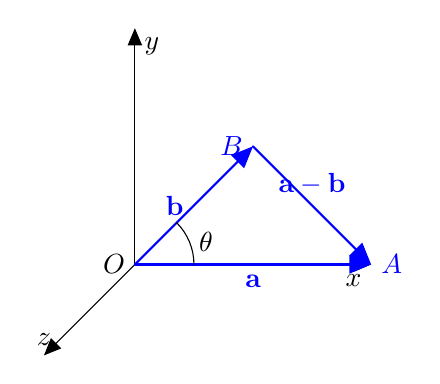
\begin{tikzpicture}[line cap=round,line join=round,>=triangle 45, scale=1.5]
			% Axes
			\draw[->] (0,0,0) -- (2,0,0) node[anchor=north east]{$x$};
			\draw[->] (0,0,0) -- (0,2,0) node[anchor=north west]{$y$};
			\draw[->] (0,0,0) -- (0,0,2) node[anchor=south]{$z$};
			
			% Vectors a, b, and a-b
			\draw[->, thick, blue] (0,0,0) -- (2,0,0) node[midway, below]{$\mathbf{a}$} node[anchor=west]{$A$};
			\draw[->, thick, blue] (0,0,0) -- (1,1,0) node[midway, left]{$\mathbf{b}$} node[anchor=east]{$B$};
			\draw[->, thick, blue] (1,1,0) -- (2,0,0) node[midway, above]{$\mathbf{a-b}$};
			
			% Angle label theta
			\draw (0.5,0,0) arc[start angle=0,end angle=45,radius=0.5] node[midway, right]{$\theta$};
			
			% Origin O
			\node[anchor=east] at (0,0,0) {$O$};
			
		\end{tikzpicture}
		\[ |AB|^{2} = |OA|^{2} + |OB|^{2} - 2 |OA| |OB| \cos \theta \] 
	\end{center}

	Corollary: If $\theta$ is the angle between nonzero vectors $\mathbf{a}$ and $\mathbf{b}$, then 
	\begin{center}
		\[ \cos(\theta)  = \frac{\mathbf{a} \cdot \mathbf{b} }{|\mathbf{a}| |\mathbf{b}| } \] 
	\end{center}
}

\ntimg{
	Two vectors $\mathbf{a}$ and $\mathbf{b}$ are orthogonal if an only if $\mathbf{a} \cdot \mathbf{b} = 0$
}

\ex{Direction Angles and Cosines}{
	The \textbf{direction angles} of a nonzero vector $\mathbf{a}$ are the angles $\alpha$, $\beta$, and $\gamma$ (in the interval $[0, \pi]$) that $\mathbf{a}$ makes with the positive $x$-, $y$-, and $z$-axes, respectively .

	The cosines of these direction angles, $\cos \alpha$, $\cos \beta$, and $\cos \gamma$, are called the \textbf{direction cosines} of the vector $\mathbf{a}$. Using Corollary 6 with $\mathbf{b}$ replaced by $\mathbf{i}$, we obtain:

	\[ \cos \alpha = \frac{\mathbf{a} \cdot \mathbf{i}}{|\mathbf{a}||\mathbf{i}|} = \frac{a_1}{|\mathbf{a}|} \tag{1} \]

	Similarly, we also have:
	\[ \cos \beta = \frac{a_2}{|\mathbf{a}|} \quad \text{and} \quad \cos \gamma = \frac{a_3}{|\mathbf{a}|} \tag{2} \]
	By squaring the expressions in Equations 8 and 9 and adding, we see that:
	\[ \cos^2 \alpha + \cos^2 \beta + \cos^2 \gamma = 1 \tag{3} \]
	We can also use Equations 8 and 9 to write:
	\[ \mathbf{a} = \langle a_1, a_2, a_3 \rangle = \langle |\mathbf{a}| \cos \alpha, |\mathbf{a}| \cos \beta, |\mathbf{a}| \cos \gamma \rangle
	= |\mathbf{a}| \langle \cos \alpha, \cos \beta, \cos \gamma \rangle \]
	Therefore,
	\[ \frac{1}{|\mathbf{a}|} \mathbf{a} = \langle \cos \alpha, \cos \beta, \cos \gamma \rangle \tag{4} \]
	which says that the direction cosines of $\mathbf{a}$ are the components of the unit vector in the direction of $\mathbf{a}$.

}

\defrose{Projections}{
	TThe \textbf{scalar projection} of $\mathbf{b}$ onto $\mathbf{a}$ (also called the \textbf{component of $\mathbf{b}$ along $\mathbf{a}$}) is defined to be the signed magnitude of the vector projection, which is the number $|\mathbf{b}| \cos \theta$, where $\theta$ is the angle between $\mathbf{a}$ and $\mathbf{b}$.
	This is denoted by $\text{comp}_{\mathbf{a}} \mathbf{b}$. Observe that it is negative if $\pi/2 < \theta \leq \pi$. The equation
	\[ 	\mathbf{a} \cdot \mathbf{b} = |\mathbf{a}| |\mathbf{b}| \cos \theta = |\mathbf{a}| (|\mathbf{b}| \cos \theta) \]
	shows that the dot product of $\mathbf{a}$ and $\mathbf{b}$ can be interpreted as the length of $\mathbf{a}$ times the scalar projection of $\mathbf{b}$ onto $\mathbf{a}$. Since
	\[ 	|\mathbf{b}| \cos \theta = \frac{\mathbf{a} \cdot \mathbf{b}}{|\mathbf{a}|} = \frac{\mathbf{a}}{|\mathbf{a}|} \cdot \mathbf{b} \]
	the component of $\mathbf{b}$ along $\mathbf{a}$ can be computed by taking the dot product of $\mathbf{b}$ with the unit vector in the direction of $\mathbf{a}$. We summarize these ideas as follows.
	\\
	\textbf{Scalar projection of $\mathbf{b}$ onto $\mathbf{a}$:} \quad $\text{comp}_{\mathbf{a}} \mathbf{b} = \frac{\mathbf{a} \cdot \mathbf{b}}{|\mathbf{a}|}$


	\textbf{Vector projection of $\mathbf{b}$ onto $\mathbf{a}$:} \quad $\text{proj}_{\mathbf{a}} \mathbf{b} = \left( \frac{\mathbf{a} \cdot \mathbf{b}}{|\mathbf{a}|^2} \right) \mathbf{a} = \frac{\mathbf{a} \cdot \mathbf{b}}{|\mathbf{a}|^2} \mathbf{a}$
}


\section{12.4 Notes (Cross Product)}

\defrose{Cross Product}{
	GGiven two nonzero vectors $\mathbf{a} = \langle a_1, a_2, a_3 \rangle$ and $\mathbf{b} = \langle b_1, b_2, b_3 \rangle$, suppose that a nonzero vector $\mathbf{c} = \langle c_1, c_2, c_3 \rangle$ is perpendicular to both $\mathbf{a}$ and $\mathbf{b}$. Then $\mathbf{a} \cdot \mathbf{c} = 0$ and $\mathbf{b} \cdot \mathbf{c} = 0$, and so:

	\begin{align}
	a_1c_1 + a_2c_2 + a_3c_3 &= 0 \tag{1} \\
	b_1c_1 + b_2c_2 + b_3c_3 &= 0 \tag{2}
	\end{align}

	To eliminate $c_3$, we multiply (1) by $b_3$ and (2) by $a_3$ and subtract:

	\[ (a_1b_3 - a_3b_1)c_1 + (a_2b_3 - a_3b_2)c_2 = 0 \tag{3} \]

	Equation (3) has the form $pc_1 + qc_2 = 0$, for which an obvious solution is $c_1 = q$ and $c_2 = -p$. So, a solution of (3) is:

	\begin{align*}
		c_1 &= a_2b_3 - a_3b_2 \\
		c_2 &= a_3b_1 - a_1b_3
	\end{align*}

	Substituting these values into (1) and (2), we then get:

	\[ 	c_3 = a_1b_2 - a_2b_1 	\]

	This means that a vector perpendicular to both $\mathbf{a}$ and $\mathbf{b}$ is:

	\[ 	\langle c_1, c_2, c_3 \rangle = \langle a_2b_3 - a_3b_2, a_3b_1 - a_1b_3, a_1b_2 - a_2b_1 \rangle \]

	The resulting vector is called the \textbf{cross product} of $\mathbf{a}$ and $\mathbf{b}$ and is denoted by $\mathbf{a} \times \mathbf{b}$.

}

\defrose{Cross Product of two vectors}{
	IIf $\mathbf{a} = \langle a_{1}, a_{2}, a_{3} \rangle $ and $\mathbf{b} = \langle b_{1}, b_{2}, b_{3} \rangle $ 
	then the \textbf{cross product} of \textbf{a} and \textbf{b} is: 
	\begin{center}
		\[ \mathbf{a} \times \mathbf{b} = \langle a_{2}b_{3} - a_{3}b_{2}, a_{3}b_{1} - a_{1}b_{3}, a_{1}b_{2} - a_{2}b_{1} \rangle \] 
	\end{center}
}

\ntimg{Determinant of order 2: 
	\begin{center}
		\[ \begin{vmatrix}
		a & b \\
		c & d
		\end{vmatrix}
		= ad - bc \]
	\end{center}
}

\ntimg{Determinant of order 3: 
	\[ 
	\begin{vmatrix}
	a_1 & a_2 & a_3 \\
	b_1 & b_2 & b_3 \\
	c_1 & c_2 & c_3
	\end{vmatrix}
	= a_1
	\begin{vmatrix}
	b_2 & b_3 \\
	c_2 & c_3
	\end{vmatrix}
	- a_2
	\begin{vmatrix}
	b_1 & b_3 \\
	c_1 & c_3
	\end{vmatrix}
	+ a_3
	\begin{vmatrix}
	b_1 & b_2 \\
	c_1 & c_2
	\end{vmatrix}
	\]
}

\defrose{Second definition of cross product}{
	AArithmetic Definition: 
	\begin{center}
		\[ a \times b = \left[ \begin{matrix}
			i & j & k  \\
			a_{1} & a_{2} & a_{3} \\
			b_{1} & b_{2} & b_{3} \\
		\end{matrix}\right] = |a||b| \sin(\theta) \] 
		\[ \left[ \begin{matrix}
			a_{2} & a_{3} \\
			b_{2} & b_{3}  \\
		\end{matrix}\right] i - \left[ \begin{matrix}
			a_{1} & a_{3} \\
			b_{1} & b_{3}  \\
		\end{matrix}\right] j + \left[ \begin{matrix}
			a_{1} & a_{2} \\
			b_{1} & b_{2} k  \\
		\end{matrix}\right]\] 
		\[ = (a_{2}b_{3} - a_{3}b_{2}) i - (a_{1}b_{3} - a_{3}b_{1}) j + (a_{1} b_{2} - a_{2}b_{1}) k \]\
	\end{center}

	The vector \textbf{a} $\times$ \textbf{b} is orthogonal to both \textbf{a} and \textbf{b} 
}

\exrose{Proof that \textbf{a} $\times$ \textbf{b} is orthogonal to both \textbf{a}}{
	\begin{align*}
		(\mathbf{a} \times \mathbf{b}) \cdot \mathbf{a} &= 
		\begin{vmatrix}
		a_2 & a_3 \\
		b_2 & b_3
		\end{vmatrix} a_1 - 
		\begin{vmatrix}
		a_1 & a_3 \\
		b_1 & b_3
		\end{vmatrix} a_2 + 
		\begin{vmatrix}
		a_1 & a_2 \\
		b_1 & b_2
		\end{vmatrix} a_3 \\
		&= a_1(a_2b_3 - a_3b_2) - a_2(a_1b_3 - a_3b_1) + a_3(a_1b_2 - a_2b_1) \\
		&= a_1a_2b_3 - a_1a_3b_2 - a_2a_1b_3 + a_2a_3b_1 + a_3a_1b_2 - a_3a_2b_1 \\
		&= 0
	\end{align*}
}

\defrose{sin definition of cross product}{
	IIf $\theta$ is the angle between \textbf{a} and \textbf{b} (so $0 \leq \theta \leq \pi$), then 
	the length of the cross product \textbf{a} $\times$ \textbf{b} is given by: 
	\[ |\mathbf{a} \times \mathbf{b} | = |\mathbf{a}| |\mathbf{b}| \sin(\theta) \]
	Proof: 
	\begin{align*}
		|\mathbf{a} \times \mathbf{b}|^2 &= (a_2b_3 - a_3b_2)^2 + (a_3b_1 - a_1b_3)^2 + (a_1b_2 - a_2b_1)^2 \\
		\\
		&= a_2^2b_3^2 - 2a_2a_3b_2b_3 + a_3^2b_2^2 + a_3^2b_1^2 - 2a_1a_3b_1b_3 + a_1^2b_3^2 + a_1^2b_2^2 - 2a_1a_2b_1b_2 + a_2^2b_1^2 \\
		\\
		&= (a_1^2 + a_2^2 + a_3^2)(b_1^2 + b_2^2 + b_3^2) - (a_1b_1 + a_2b_2 + a_3b_3)^2 \\
		\\
		&= |\mathbf{a}|^2 |\mathbf{b}|^2 - (\mathbf{a} \cdot \mathbf{b})^2 \\
		\\
		&= |\mathbf{a}|^2 |\mathbf{b}|^2 - |\mathbf{a}|^2 |\mathbf{b}|^2 \cos^2 \theta \quad \text{(by Theorem 12.3.3)} \\
		\\
		&= |\mathbf{a}|^2 |\mathbf{b}|^2 (1 - \cos^2 \theta) \\
		\\
		&= |\mathbf{a}|^2 |\mathbf{b}|^2 \sin^2 \theta
	\end{align*}

	Taking square roots and observing that \(\sqrt{\sin^2 \theta} = \sin \theta\) because \(\sin \theta \geq 0\) when \(0 \leq \theta \leq \pi\), we have
	\[ |\mathbf{a} \times \mathbf{b}| = |\mathbf{a}| |\mathbf{b}| \sin \theta \]
}

\ntimg{
	Two nonzero vectors \textbf{a} and \textbf{b} are parallel if and only if 
	\[ \mathbf{a} \times \mathbf{b} = 0 \] 
}

\exrose{Geometric interpretation of $|\mathbf{a} \times \mathbf{b}| = |\mathbf{a}| |\mathbf{b}| \sin \theta$}{
	If \textbf{a} and \textbf{b} are represented by directed line segments with the same inital point, then they determine 
	a parallelogram with base $|\mathbf{a}|$, altitude $\mathbf{b}\sin(\theta)$ and area 
	\[ A = |\mathbf{a}|(|\mathbf{b}| \sin \theta ) = |\mathbf{a} \times \mathbf{b}|  \] 
	Thus we have the following way of interpreting the magnitude of a cross product: \\
	The length of the cross product of \textbf{a} $\times$ \textbf{b} is equal to the area of the 
	parallelogram determined by \textbf{a} and \textbf{b} 
}

\ntimg{
	If we apply the following theorem:

	The vector \(\mathbf{a} \times \mathbf{b}\) is orthogonal to both \(\mathbf{a}\) and \(\mathbf{b}\), and 
	\[ 	|\mathbf{a} \times \mathbf{b}| = |\mathbf{a}| |\mathbf{b}| \sin \theta \]
	to the standard basis vectors \(\mathbf{i}, \mathbf{j}, \mathbf{k}\) using \(\theta = \frac{\pi}{2}\), we obtain

	\[
	\begin{aligned}
		\mathbf{i} \times \mathbf{j} &= \mathbf{k} \quad &\mathbf{j} \times \mathbf{k} &= \mathbf{i} \quad &\mathbf{k} \times \mathbf{i} &= \mathbf{j} \\
		\mathbf{j} \times \mathbf{i} &= -\mathbf{k} \quad &\mathbf{k} \times \mathbf{j} &= -\mathbf{i} \quad &\mathbf{i} \times \mathbf{k} &= -\mathbf{j}
	\end{aligned}
	\]
}


\ntimg{
	If \(\mathbf{a}\), \(\mathbf{b}\), and \(\mathbf{c}\) are vectors and \(c\) is a scalar, then
	\begin{enumerate}
		\item \(\mathbf{a} \times \mathbf{b} = -\mathbf{b} \times \mathbf{a}\)
		\item \((c\mathbf{a}) \times \mathbf{b} = c(\mathbf{a} \times \mathbf{b}) = \mathbf{a} \times (c\mathbf{b})\)
		\item \(\mathbf{a} \times (\mathbf{b} + \mathbf{c}) = \mathbf{a} \times \mathbf{b} + \mathbf{a} \times \mathbf{c}\)
		\item \((\mathbf{a} + \mathbf{b}) \times \mathbf{c} = \mathbf{a} \times \mathbf{c} + \mathbf{b} \times \mathbf{c}\)
		\item \(\mathbf{a} \cdot (\mathbf{b} \times \mathbf{c}) = (\mathbf{a} \times \mathbf{b}) \cdot \mathbf{c}\)
		\item \(\mathbf{a} \times (\mathbf{b} \times \mathbf{c}) = (\mathbf{a} \cdot \mathbf{c})\mathbf{b} - (\mathbf{a} \cdot \mathbf{b})\mathbf{c}\)
	\end{enumerate}
}

\exrose{Proof of property 5 of cross products}{
	If \(\mathbf{a} = \langle a_1, a_2, a_3 \rangle\), \(\mathbf{b} = \langle b_1, b_2, b_3 \rangle\), and \(\mathbf{c} = \langle c_1, c_2, c_3 \rangle\), then: 
	\begin{align*}
		\mathbf{a} \cdot (\mathbf{b} \times \mathbf{c}) &= a_1(b_2c_3 - b_3c_2) + a_2(b_3c_1 - b_1c_3) + a_3(b_1c_2 - b_2c_1)\\ 
		\\
		&= a_1b_2c_3 - a_1b_3c_2 + a_2b_3c_1 - a_2b_1c_3 + a_3b_1c_2 - a_3b_2c_1 \\
		\\
		&= (a_2b_3 - a_3b_2)c_1 + (a_3b_1 - a_1b_3)c_2 + (a_1b_2 - a_2b_1)c_3 \\
		\\
		&= (\mathbf{a} \times \mathbf{b}) \cdot \mathbf{c} \\
	\end{align*}
}

\defrose{Triple Products}{ 
	TThe product \(\mathbf{a} \cdot (\mathbf{b} \times \mathbf{c})\) that occurs in Property 5 is called the \textit{scalar triple product} of the vectors \(\mathbf{a}\), \(\mathbf{b}\), and \(\mathbf{c}\). 

	\[ 	\mathbf{a} \cdot (\mathbf{b} \times \mathbf{c}) = 
	\begin{vmatrix}
	a_1 & a_2 & a_3 \\
	b_1 & b_2 & b_3 \\
	c_1 & c_2 & c_3
	\end{vmatrix} \]
	
	The geometric significance of the scalar triple product can be seen by considering the parallelepiped determined by the vectors \(\mathbf{a}\), \(\mathbf{b}\), and \(\mathbf{c}\). The area of the base parallelogram is \(A = |\mathbf{b} \times \mathbf{c}|\). If \(\theta\) is the angle between \(\mathbf{a}\) and \(\mathbf{b} \times \mathbf{c}\), then the height \(h\) of the parallelepiped is \(h = |\mathbf{a}| |\cos \theta|\). (We must use \(|\cos \theta|\) instead of \(\cos \theta\) in case \(\theta > \pi / 2\).) Therefore, the volume of the parallelepiped is
	
	\[ 	V = A h = |\mathbf{b} \times \mathbf{c}| |\mathbf{a}| |\cos \theta| = |\mathbf{a} \cdot (\mathbf{b} \times \mathbf{c})| \]
	
	Thus, we have proved the following formula: 
	The volume of the parallelepiped determined by the vectors \textbf{a}, \textbf{b}, and \textbf{c} is the magnitude of their scalar triple product:
	\[ V = |\mathbf{a} \cdot (\mathbf{b} \times \mathbf{c})| \] 
 }
 
 \ntimg{
	If we use the formula in $V = |\mathbf{a} \cdot (\mathbf{b} \times \mathbf{c})|$ and discover that the volume of the parallelepiped
	determined by a, b, and c is 0, then the vectors must lie in the same plane; that is, they
	are coplanar
 }
 \section{12.5 Notes (Equations of Lines and Planes)}

\defrose{Hi}{
	LLikewise, a line \(L\) in three-dimensional space is determined when we know a point
	\(P_0(x_0, y_0, z_0)\) on \(L\) and a direction for \(L\), which is conveniently 
	described by a vector \(\mathbf{v}\) parallel to the line. Let \(P(x, y, z)\) be an
	arbitrary point on \(L\) and let \(\mathbf{r_0}\) and \(\mathbf{r}\) be the position
	vectors of \(P_0\) and \(P\) (that is, they have representations
	\(\overrightarrow{OP_0}\) and \(\overrightarrow{OP}\)). If \(\mathbf{a}\) is the
	vector with representation \(\overrightarrow{P_0P}\), as in Figure 1, then the
	Triangle Law for vector addition gives

	\[
	\mathbf{r} = \mathbf{r_0} + \mathbf{a}.
	\]

	\insertpng[0.25]{lines.png}
	Since \textbf{a} and \textbf{v} are parallel vectors, there is a scalar \textit{t} such that 
	$\mathbf{a} = t \mathbf{v} $ Thus  
	\[ r = r_{0} + t \mathbf{v}\] 
}

\ntimg{
	If the vector \(\mathbf{v}\) that gives the direction of the line \(L\) is written in component form as 
	\[ 	\mathbf{v} = \langle a, b, c \rangle, \]
	then we have \( t\mathbf{v} = \langle ta, tb, tc \rangle \). We can also write \(\mathbf{r} = \langle x, y, z \rangle\) and 
	\[ 	\mathbf{r}_0 = \langle x_0, y_0, z_0 \rangle, \]
	so the vector equation (1) becomes 
	\[	\langle x, y, z \rangle = \langle x_0 + ta, y_0 + tb, z_0 + tc \rangle. \]
	Two vectors are equal if and only if corresponding components are equal. Therefore we have the three scalar equations:
	\[ 	x = x_0 + at \quad y = y_0 + bt \quad z = z_0 + ct 	\]
}

\exrose{Line example}{
	Find a vector equation and parametric equations for the line that passes through the point \((5, 1, 3)\) and is parallel to the vector \(\mathbf{i} + 4\mathbf{j} - 2\mathbf{k}\).
	Here \(\mathbf{r}_0 = \langle 5, 1, 3 \rangle = 5\mathbf{i} + \mathbf{j} + 3\mathbf{k}\) and \(\mathbf{v} = \mathbf{i} + 4\mathbf{j} - 2\mathbf{k}\), so the vector equation (1) becomes
	\[ \mathbf{r} = (5\mathbf{i} + \mathbf{j} + 3\mathbf{k}) + t(\mathbf{i} + 4\mathbf{j} - 2\mathbf{k}) \]
	or
	\[ \mathbf{r} = (5 + t)\mathbf{i} + (1 + 4t)\mathbf{j} + (3 - 2t)\mathbf{k} \]
	Parametric equations are
	\[ x = 5 + t \quad y = 1 + 4t \quad z = 3 - 2t \]
}

\ntimg{
	In general, if a vector \(\mathbf{v} = \langle a, b, c \rangle\) is used to describe
	the direction of a line \(L\), then the numbers \(a\), \(b\), and \(c\) are called 
	\textit{direction numbers} of \(L\). Since any vector parallel to \(\mathbf{v}\) could
	 also be used, we see that any three numbers proportional to \(a\), \(b\), and \(c\) 
	could also be used as a set of direction numbers for \(L\). \\

	Another way of describing a line \(L\) is to eliminate the parameter \(t\) 
	from Equations 2. If none of \(a\), \(b\), or \(c\) is 0, we can solve each of
	 these equations for \(t\):

	\[ 	t = \frac{x - x_0}{a} \quad t = \frac{y - y_0}{b} \quad t = \frac{z - z_0}{c} \]

	Equating the results, we obtain
	\[ \frac{x - x_0}{a} = \frac{y - y_0}{b} = \frac{z - z_0}{c} \]

	These equations are called symetric equations of \(L\) 
}

\defrose{Line segment}{
	TThe line segment from $r_{0}$ to $r_{1}$ is given by the vector equation 
	\[ \mathbf{r}(t) = (1-t)\mathbf{r_{0}} + tr_{1} \quad 0 \leq t \leq 1\] 
}

\defrose{Planes}{
	AA plane in space is determined by a point $P_0(x_0, y_0, z_0)$ in the plane and a
	vector $\mathbf{n}$ that is orthogonal to the plane. This orthogonal vector
	$\mathbf{n}$ is called a \textbf{normal vector}. Let $P(x, y, z)$ be an arbitrary
	 point in the plane, and let $\mathbf{r_0}$ and $\mathbf{r}$ be the position vectors
	of $P_0$ and $P$. Then the vector $\mathbf{r - r_0}$ is represented by
	$\overrightarrow{P_0P}$.

	The normal vector $\mathbf{n}$ is orthogonal to every vector in the given plane. 
	In particular, $\mathbf{n}$ is orthogonal to $\mathbf{r - r_0}$ and so we have
	\begin{equation}
		\mathbf{n} \cdot (\mathbf{r} - \mathbf{r_0}) = 0
	\end{equation}
	which can be rewritten as
	\begin{equation}
		\mathbf{n} \cdot \mathbf{r} = \mathbf{n} \cdot \mathbf{r_0}
	\end{equation}
	These can be reffered to as the \textbf{vector equation of the plane}

	To obtain a scalar equation for the plane, we write \textbf{n} $ = \langle a, b, c \rangle, 
	\mathbf{r} = \langle x, y, x \rangle$, and $\mathbf{r}_{0} = \langle x_{0}, y_{0}, z_{0} \rangle$. then the 
	vector equation becomes: 
	\[ \langle a, b, c \rangle \cdot \langle x - x_{0}, y - y_{0}, z - z_{0} \rangle = 0 \] 

	Expanding the left side of this equation gives the following: \\
	A \textbf{scalar equation of the plane} through the point $P_{0}(x_{0}, y_{0}, z_{0})$ with normal vector 
	\textbf{n} $ = \langle a, b, c \rangle$ is 
	\[ a(x - x_{0}) + b(y - y_{0}) + c(z - z_{0}) = 0 \]
	by colecting terms can be rewritten as: 
	\[ ax + by + cz + d = 0 \]    
}

\defrose{Distance of a plane}{
	IIn order to find a formula for the distance $D$ from a point $P_1(x_1, y_1, z_1)$ to the plane $ax + by + cz + d = 0$, we let $P_0(x_0, y_0, z_0)$ be any point in the given plane and $\mathbf{b}$ be the vector corresponding to $\overrightarrow{P_0 P_1}$. Then

	\[ 	\mathbf{b} = \langle x_1 - x_0, y_1 - y_0, z_1 - z_0 \rangle \]
	
	\begin{center}
		\insertpng[0.6]{distances.png}
	\end{center}

	From Figure, you can see that the distance $D$ from $P_1$ to the plane is equal to the absolute value of the scalar projection of $\mathbf{b}$ onto the normal vector $\mathbf{n} = \langle a, b, c \rangle$. Thus,

	\[ 	D = |\text{comp}_{\mathbf{n}} \mathbf{b}| = \frac{|\mathbf{n} \cdot \mathbf{b}|}{|\mathbf{n}|} \]

	\[ 	= \frac{|a(x_1 - x_0) + b(y_1 - y_0) + c(z_1 - z_0)|}{\sqrt{a^2 + b^2 + c^2}} \]

	\[	= \frac{|(a x_1 + b y_1 + c z_1) - (a x_0 + b y_0 + c z_0)|}{\sqrt{a^2 + b^2 + c^2}} \]
}

\section{12.6 Reading Notes (Cylinders and Quadric Surfaces)}

\defrose{Cylinder}{
	AA cylinder is a surface that consists of all lines (called rulings) that are parallel to a
	given line and pass through a given plane curve.
}

\defrose{Quadric Surfaces}{
	AA  Quadric Surface is the graph of a second-degree equation in three variables $x$, $y$, and $z$. The most general such equation is
	\[ Ax^2 + By^2 + Cz^2 + Dxy + Eyz + Fzx + Gx + Hy + Iz + J = 0 \]

	where $A$, $B$, $C$, $\dots$, $J$ are constants, but by translation and rotation it can be brought into one of the two \textit{standard forms}

	\[ Ax^2 + By^2 + Cz^2 + J = 0 \quad \text{or} \quad Ax^2 + By^2 + Iz = 0 \] 
}

\exrose{Graphs of Quadric Surfaces PT 1}{
	Ellipsoid: 
	\insertpng[0.7]{ellipsoid.png}
	\[ \frac{x^2}{a^2} + \frac{y^2}{b^2} + \frac{z^2}{c^2} = 1 \] 
	All traces are ellipses. If \(a = b = c\), the ellipsoid is a sphere. \\
	\insertpng[0.7]{EllipticParaboloid.png}
	\[ \frac{z}{c} = \frac{x^2}{a^2} + \frac{y^2}{b^2} \] 
	Horizontal traces are ellipses. Vertical traces are parabolas. The variable raised to the first power indicates the axis of the paraboloid. \\
	\insertpng[0.7]{HyperbolicParaboloid}
	\[ \frac{z}{c} = \frac{x^2}{a^2} - \frac{y^2}{b^2} \] 
	Horizontal traces are hyperbolas. Vertical traces are parabolas. The case where \(c < 0\) is illustrated. \\
}

\exrose{Quadric Surfaces Pt 2}{
	\insertpng[0.7]{Cone.png}
	\[ \frac{z^2}{c^2} = \frac{x^2}{a^2} + \frac{y^2}{b^2} \] 
	Horizontal traces are ellipses. Vertical traces in the planes \(x = k\) and \(y = k\) are hyperbolas if \(k \neq 0\) but are pairs of lines if \(k = 0\). \\
	\insertpng[0.7]{HyperboloidofOneSheet.png}
	\[ \frac{x^2}{a^2} + \frac{y^2}{b^2} - \frac{z^2}{c^2} = 1 \] 
	Horizontal traces are ellipses. Vertical traces are hyperbolas. The axis of symmetry corresponds to the variable whose coefficient is negative. \\
	\insertpng[0.7]{HyperboloidofTwoSheets.png}
	\[ -\frac{x^2}{a^2} - \frac{y^2}{b^2} + \frac{z^2}{c^2} = 1 \] 
	Horizontal traces in \(z = k\) are ellipses if \(k > c\) or \(k < -c\). Vertical traces are hyperbolas. The two minus signs indicate two sheets. \\
}

\chapter{}
\section{13.1 Reading Notes(Vector Functions and Space Curves)}

\defrose{Vector Value Functions}{
	AA \textbf{vector-valued function}, or \textbf{vector function}, is simply a function whose
	domain is a set of real numbers and whose range is a set of vectors. We are most 
	interested in vector functions r whose values are three-dimensional vectors. If
	$f(t)$, $g(t)$, and $h(t)$ are the components of the vector \textbf{r}$(t)$, then $f$ , $g$, and $h$ are real-valued
	functions called the \textbf{component functions} of r and we can write

	\[ \mathbf{r}(t) = \langle f(t), g(t), h(t) \rangle = f(t) \mathbf{i} + g(t) \mathbf{j} + h(t) \mathbf{k} \]
	We use the letter \( t \) to denote the independent variable because it represents time in most applications of vector functions.
}

\defrose{Limit of Vectors}{
	TThe \textbf{limit} of a vector function \(\mathbf{r}\) is defined by taking the limits of its component functions as follows.

    If $(\mathbf{r}(t) = \langle f(t), g(t), h(t) \rangle)$, then
    \[ \lim_{t \to a} \mathbf{r}(t) = \left\langle \lim_{t \to a} f(t), \lim_{t \to a} g(t), \lim_{t \to a} h(t) \right\rangle \]
    provided the limits of the component functions exist.
}

\defrose{Space Curves}{
	There is a close connection between continuous vector functions and space curves. Suppose that \( f \), \( g \), and \( h \) are continuous real-valued functions on an interval \( I \). Then the set \( C \) of all points \( (x, y, z) \) in space, where
	\[ x = f(t) \quad y = g(t) \quad z = h(t) \]
	and $( t )$ varies throughout the interval \( I \), is called a \textbf{space curve}.
    The equations in are called \textbf{parametric equations of} \( C \) and \( t \) is called a \textbf{parameter}.
}

\section{13.2 Notes (Derivatives and Integrals of Vector Functions)}

\defrose{Derivatives}{
	TThe derivative \(\mathbf{r}'\) of a vector function \(\mathbf{r}\) is defined in much the same way as for real-valued functions:
	\[ \frac{d\mathbf{r}}{dt} = \mathbf{r}'(t) = \lim_{h \to 0} \frac{\mathbf{r}(t+h) - \mathbf{r}(t)}{h} \]
}

\defrose{Derivatives of vectors pt 2}{
	The following theorem gives us a convenient method for computing the derivative of a vector function \(\mathbf{r}\): just differentiate each component of \(\mathbf{r}\).
	\textbf{Theorem} If \(\mathbf{r}(t) = \langle f(t), g(t), h(t) \rangle = f(t) \mathbf{i} + g(t) \mathbf{j} + h(t) \mathbf{k}\), where \(f\), \(g\), and \(h\) are differentiable functions, then
	\[ \mathbf{r}'(t) = \langle f'(t), g'(t), h'(t) \rangle = f'(t) \mathbf{i} + g'(t) \mathbf{j} + h'(t) \mathbf{k} \]
}

\exrose{Proof of Definition 2.2.2}{
	\[ \mathbf{r}'(t) = \lim_{\Delta t \to 0} \frac{1}{\Delta t} [\mathbf{r}(t + \Delta t) - \mathbf{r}(t)] \]
	\[ 	= \lim_{\Delta t \to 0} \frac{1}{\Delta t} [\langle f(t + \Delta t), g(t + \Delta t), h(t + \Delta t) \rangle - \langle f(t), g(t), h(t) \rangle] \]
	\[ 	= \lim_{\Delta t \to 0} \left\langle \frac{f(t + \Delta t) - f(t)}{\Delta t}, \frac{g(t + \Delta t) - g(t)}{\Delta t}, \frac{h(t + \Delta t) - h(t)}{\Delta t} \right\rangle \]
	\[ 	= \left\langle \lim_{\Delta t \to 0} \frac{f(t + \Delta t) - f(t)}{\Delta t}, \lim_{\Delta t \to 0} \frac{g(t + \Delta t) - g(t)}{\Delta t}, \lim_{\Delta t \to 0} \frac{h(t + \Delta t) - h(t)}{\Delta t} \right\rangle \]
	\[ 	= \langle f'(t), g'(t), h'(t) \rangle \]
	A unit vector that has the same direction as the tangent vector is called the \textbf{unit tangent vector} \(\mathbf{T}\) and is defined by
	\[ 	\mathbf{T}(t) = \frac{\mathbf{r}'(t)}{|\mathbf{r}'(t)|} \]
}

\defrose{Differentiation Rules}{
	PProof:
	\textbf{Theorem} Suppose \(\mathbf{u}\) and \(\mathbf{v}\) are differentiable vector functions, \(c\) is a scalar, and \(f\) is a real-valued function. Then
	\begin{enumerate}
		\item \(\frac{d}{dt} [\mathbf{u}(t) + \mathbf{v}(t)] = \mathbf{u}'(t) + \mathbf{v}'(t)\)
		\item \(\frac{d}{dt} [c\mathbf{u}(t)] = c\mathbf{u}'(t)\)
		\item \(\frac{d}{dt} [f(t)\mathbf{u}(t)] = f'(t)\mathbf{u}(t) + f(t)\mathbf{u}'(t)\)
		\item \(\frac{d}{dt} [\mathbf{u}(t) \cdot \mathbf{v}(t)] = \mathbf{u}'(t) \cdot \mathbf{v}(t) + \mathbf{u}(t) \cdot \mathbf{v}'(t)\)
		\item \(\frac{d}{dt} [\mathbf{u}(t) \times \mathbf{v}(t)] = \mathbf{u}'(t) \times \mathbf{v}(t) + \mathbf{u}(t) \times \mathbf{v}'(t)\)
		\item \(\frac{d}{dt} [\mathbf{u}(f(t))] = f'(t) \mathbf{u}'(f(t))\) \hfill \textcolor{blue}{(Chain Rule)}
	\end{enumerate}
}

\ntimg{
	We use Formula 4 to prove the following theorem.
	\textbf{Theorem} If \(|\mathbf{r}(t)| = c\) (a constant), then \(\mathbf{r}'(t)\) is orthogonal to \(\mathbf{r}(t)\) for all \(t\).
}

\defrose{Interation of Vectors}{
	TThe \textbf{definite integral} of a continuous vector function \(\mathbf{r}(t)\) can be defined in much the same way as for real-valued functions except that the integral is a vector. But then we can express the integral of \(\mathbf{r}\) in terms of the integrals of its component functions \(f\), \(g\), and \(h\) as follows. (We use the notation of Chapter 5.)

	\[ \int_a^b \mathbf{r}(t) \, dt = \lim_{n \to \infty} \sum_{j=1}^{n} \mathbf{r}(t_j^*) \, \Delta t \]
	\[ = \lim_{n \to \infty} \left[ \left( \sum_{i=1}^{n} f(t_i^*) \, \Delta t \right) \mathbf{i} + \left( \sum_{i=1}^{n} g(t_i^*) \, \Delta t \right) \mathbf{j} + \left( \sum_{i=1}^{n} h(t_i^*) \, \Delta t \right) \mathbf{k} \right] \]
	and so
	\[ \int_a^b \mathbf{r}(t) \, dt = \left( \int_a^b f(t) \, dt \right) \mathbf{i} + \left( \int_a^b g(t) \, dt \right) \mathbf{j} + \left( \int_a^b h(t) \, dt \right) \mathbf{k} \]
	This means that we can evaluate an integral of a vector function by integrating each component function.

	We can extend the Fundamental Theorem of Calculus to continuous vector functions as follows:
	\[ 	\int_a^b \mathbf{r}(t) \, dt = \mathbf{R}(t) \Big|_a^b = \mathbf{R}(b) - \mathbf{R}(a) \]
	where \(\mathbf{R}\) is an antiderivative of \(\mathbf{r}\), that is, \(\mathbf{R}'(t) = \mathbf{r}(t)\). We use the notation \(\int \mathbf{r}(t) \, dt\) for indefinite integrals (antiderivatives).
	}




\end{document}
